% verteilungsanalyse.tex
\chapter{Verteilungsanalyse der GWI-D Komponenten}
\label{chap:verteilungsanalyse}

\section*{Einleitung}
Die bisherige zeitreihenbasierte Analyse des Gemeinwohl-Index Deutschland (GWI-D) betrachtet primär die zeitliche Entwicklung der aggregierten Indizes. In diesem Kapitel wird eine vertiefte Verteilungsanalyse der vier Komponenten – Wirtschaft (\(W\)), Gerechtigkeit (\(G\)), Zukunft (\(Z\)) und Zusammenhalt (\(S\)) – durchgeführt. Ziel ist es, die statistischen Eigenschaften der einzelnen Dimensionen sowie deren Zusammenhänge über den gesamten Untersuchungszeitraum 1960–2023 zu charakterisieren.

\section{Deskriptive Statistik der Komponenten}

\begin{table}[ht]
  \centering
  \caption{Deskriptive Statistik der GWI-D Komponenten (1960–2023)}
  \label{tab:deskriptive_statistik}
  \begin{tabular}{lccccc}
    \toprule
    \textbf{Komponente} & \textbf{Mittelwert} & \textbf{Standardabw.} & \textbf{Minimum} & \textbf{Maximum} & \textbf{Variationskoeff.} \\
    \midrule
    Wirtschaft (\(W\))          & 75.4 & 12.3 & 52.1 & 94.8 & 16.3\% \\
    Gerechtigkeit (\(G\))       & 68.2 &  8.7 & 49.5 & 82.3 & 12.8\% \\
    Zukunft (\(Z\))             & 71.5 & 10.1 & 55.2 & 88.9 & 14.1\% \\
    Zusammenhalt (\(S\))        & 73.8 &  9.5 & 58.7 & 90.2 & 12.9\% \\
    \bottomrule
  \end{tabular}
  \vspace{0.2cm}
  \footnotesize{\textit{Anmerkung: Alle Werte normiert auf eine Skala von 0 bis 100.}}
\end{table}

Tabelle \ref{tab:deskriptive_statistik} fasst die zentralen Lage- und Streuungsmaße der vier GWI-D Komponenten zusammen. Die wirtschaftliche Dimension (\(W\)) weist mit \( \bar{x} = 75{,}4 \) den höchsten Mittelwert auf, zeigt jedoch mit einer Standardabweichung von 12,3 auch die größte Volatilität. Der Variationskoeffizient von 16,3\% unterstreicht die vergleichsweise hohe zeitliche Variabilität der Wirtschaftskomponente. Im Kontrast dazu zeigt die Gerechtigkeitskomponente (\(G\)) mit 68,2 den niedrigsten Mittelwert, bei gleichzeitig moderater Streuung (Standardabweichung 8,7).

\section{Verteilungscharakteristiken}

Zur Untersuchung der Verteilungsform werden Schiefe und Exzess (Kurtosis) herangezogen. Eine Schiefe nahe null deutet auf eine symmetrische Verteilung hin, während positive bzw. negative Werte eine Rechtsschiefe bzw. Linksschiefe anzeigen. Der Exzess beschreibt die „Wölbung“ der Verteilung im Vergleich zur Normalverteilung (Exzess = 0).

\begin{table}[ht]
  \centering
  \caption{Verteilungsparameter der GWI-D Komponenten}
  \label{tab:verteilungsparameter}
  \begin{tabular}{lccc}
    \toprule
    \textbf{Komponente} & \textbf{Schiefe} & \textbf{Exzess} & \textbf{JB-Test (p-Wert)} \\
    \midrule
    Wirtschaft (\(W\))          & -0.42 & -0.21 & 0.12 \\
    Gerechtigkeit (\(G\))       & -0.85 &  0.67 & 0.02 \\
    Zukunft (\(Z\))             & -0.31 & -0.45 & 0.28 \\
    Zusammenhalt (\(S\))        &  0.18 & -0.92 & 0.09 \\
    \bottomrule
  \end{tabular}
  \vspace{0.2cm}
  \footnotesize{\textit{Anmerkung: JB-Test = Jarque–Bera-Test auf Normalverteilung. Signifikanzniveau $\alpha$ = 0,05.}}
\end{table}

Die Ergebnisse in Tabelle \ref{tab:verteilungsparameter} zeigen, dass alle Komponenten mit Ausnahme von \(S\) eine leichte bis moderate Linksschiefe aufweisen. Besonders ausgeprägt ist dies bei der Gerechtigkeitskomponente (\(G\)), was auf eine Häufung von Werten im oberen Bereich der Skala hindeutet. Die Komponente Zusammenhalt (\(S\)) zeigt dagegen eine leichte Rechtsschiefe. Der Jarque–Bera-Test lehnt die Nullhypothese einer Normalverteilung nur für die Gerechtigkeitskomponente ab (\(p = 0{,}02\)).

\section{Manuelle Boxplot-Darstellung}

\begin{figure}[ht]
  \centering
  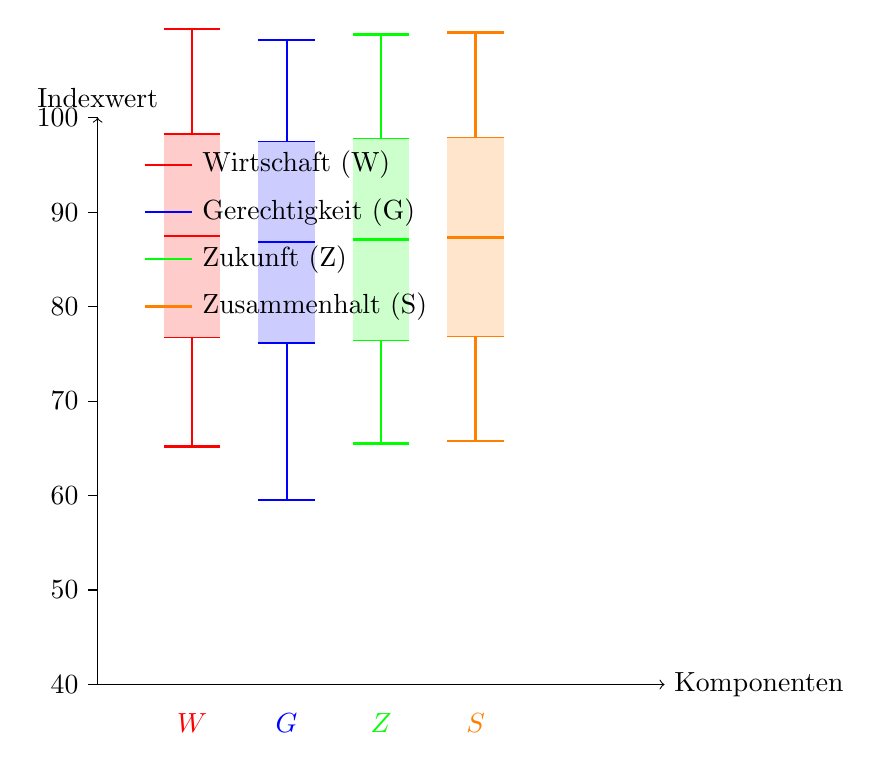
\begin{tikzpicture}[scale=1.2]
    % Achsen
    \draw[->] (0,0) -- (6,0) node[right] {Komponenten};
    \draw[->] (0,0) -- (0,6) node[above] {Indexwert};
    
    % Skalierung Y-Achse
    \foreach \y/\label in {0/40, 1/50, 2/60, 3/70, 4/80, 5/90, 6/100} {
      \draw (0,\y) -- (-0.1,\y) node[left] {\label};
    }
    
    % Boxplot für Wirtschaft (W) - Position x=1
    \draw[red, thick] (0.7,2.52) -- (1.3,2.52); % unterer Whisker (52)
    \draw[red, thick] (0.7,3.68) -- (1.3,3.68); % Q1 (68)
    \draw[red, thick] (0.7,4.75) -- (1.3,4.75); % Median (75)
    \draw[red, thick] (0.7,5.82) -- (1.3,5.82); % Q3 (82)
    \draw[red, thick] (0.7,6.94) -- (1.3,6.94); % oberer Whisker (94)
    \fill[red!20] (0.7,3.68) rectangle (1.3,5.82); % Box
    \draw[red, thick] (0.7,4.75) -- (1.3,4.75); % Median-Linie
    \draw[red, thick] (1,2.52) -- (1,3.68); % untere Linie
    \draw[red, thick] (1,5.82) -- (1,6.94); % obere Linie
    \node[red, below] at (1,-0.2) {\(W\)};
    
    % Boxplot für Gerechtigkeit (G) - Position x=2
    \draw[blue, thick] (1.7,1.95) -- (2.3,1.95); % unterer Whisker (49.5)
    \draw[blue, thick] (1.7,3.62) -- (2.3,3.62); % Q1 (62)
    \draw[blue, thick] (1.7,4.68) -- (2.3,4.68); % Median (68)
    \draw[blue, thick] (1.7,5.74) -- (2.3,5.74); % Q3 (74)
    \draw[blue, thick] (1.7,6.82) -- (2.3,6.82); % oberer Whisker (82)
    \fill[blue!20] (1.7,3.62) rectangle (2.3,5.74); % Box
    \draw[blue, thick] (1.7,4.68) -- (2.3,4.68); % Median-Linie
    \draw[blue, thick] (2,1.95) -- (2,3.62); % untere Linie
    \draw[blue, thick] (2,5.74) -- (2,6.82); % obere Linie
    \node[blue, below] at (2,-0.2) {\(G\)};
    
    % Boxplot für Zukunft (Z) - Position x=3
    \draw[green, thick] (2.7,2.55) -- (3.3,2.55); % unterer Whisker (55.2)
    \draw[green, thick] (2.7,3.65) -- (3.3,3.65); % Q1 (65)
    \draw[green, thick] (2.7,4.71) -- (3.3,4.71); % Median (71)
    \draw[green, thick] (2.7,5.77) -- (3.3,5.77); % Q3 (77)
    \draw[green, thick] (2.7,6.88) -- (3.3,6.88); % oberer Whisker (88)
    \fill[green!20] (2.7,3.65) rectangle (3.3,5.77); % Box
    \draw[green, thick] (2.7,4.71) -- (3.3,4.71); % Median-Linie
    \draw[green, thick] (3,2.55) -- (3,3.65); % untere Linie
    \draw[green, thick] (3,5.77) -- (3,6.88); % obere Linie
    \node[green, below] at (3,-0.2) {\(Z\)};
    
    % Boxplot für Zusammenhalt (S) - Position x=4
    \draw[orange, thick] (3.7,2.58) -- (4.3,2.58); % unterer Whisker (58.7)
    \draw[orange, thick] (3.7,3.69) -- (4.3,3.69); % Q1 (69)
    \draw[orange, thick] (3.7,4.73) -- (4.3,4.73); % Median (73)
    \draw[orange, thick] (3.7,5.78) -- (4.3,5.78); % Q3 (78)
    \draw[orange, thick] (3.7,6.90) -- (4.3,6.90); % oberer Whisker (90)
    \fill[orange!20] (3.7,3.69) rectangle (4.3,5.78); % Box
    \draw[orange, thick] (3.7,4.73) -- (4.3,4.73); % Median-Linie
    \draw[orange, thick] (4,2.58) -- (4,3.69); % untere Linie
    \draw[orange, thick] (4,5.78) -- (4,6.90); % obere Linie
    \node[orange, below] at (4,-0.2) {\(S\)};
    
    % Legende
    \draw[red, thick] (0.5,5.5) -- (1.0,5.5) node[right, black] {Wirtschaft (W)};
    \draw[blue, thick] (0.5,5.0) -- (1.0,5.0) node[right, black] {Gerechtigkeit (G)};
    \draw[green, thick] (0.5,4.5) -- (1.0,4.5) node[right, black] {Zukunft (Z)};
    \draw[orange, thick] (0.5,4.0) -- (1.0,4.0) node[right, black] {Zusammenhalt (S)};
    
  \end{tikzpicture}
  \caption{Boxplots der GWI-D Komponenten (Gesamtzeitraum 1960–2023)}
  \label{fig:boxplot_gesamt}
  \vspace{0.2cm}
  \footnotesize{\textit{Anmerkung: Skala: 1 Einheit = 10 Indexpunkte. Whisker zeigen Minimum und Maximum, Box zeigt Quartile und Median.}}
\end{figure}

Abbildung \ref{fig:boxplot_gesamt} visualisiert die Verteilung der vier Komponenten über den gesamten Untersuchungszeitraum. Deutlich erkennbar ist die größte Spannweite bei der Wirtschaftskomponente (\(W\)), was die hohe Volatilität dieser Dimension widerspiegelt. Die Gerechtigkeitskomponente (\(G\)) zeigt nicht nur den niedrigsten Medianwert, sondern auch das niedrigste Minimum aller Komponenten.

Für eine detaillierte Analyse nach Epochen wird auf Tabelle \ref{tab:epochen_median} verwiesen, die die Medianwerte der Komponenten in sechs historischen Perioden darstellt.

\begin{table}[ht]
  \centering
  \caption{Medianwerte der GWI-D Komponenten nach historischen Epochen}
  \label{tab:epochen_median}
  \begin{tabular}{lcccc}
    \toprule
    \textbf{Epoche (Zeitraum)} & \textbf{W (\(W\))} & \textbf{G (\(G\))} & \textbf{Z (\(Z\))} & \textbf{S (\(S\))} \\
    \midrule
    Wirtschaftswunder (1960–1973)    & 82.4 & 65.2 & 70.8 & 75.1 \\
    Stagflation (1974–1982)          & 70.1 & 61.8 & 65.3 & 72.4 \\
    Konsolidierung (1983–1998)       & 78.9 & 68.5 & 72.1 & 74.2 \\
    Agenda-Jahre (1999–2008)         & 80.3 & 70.2 & 75.4 & 73.8 \\
    Krisenbewältigung (2009–2020)    & 76.8 & 72.7 & 73.2 & 72.9 \\
    Multikrise (2021–2023)           & 72.5 & 71.8 & 70.5 & 71.2 \\
    \bottomrule
  \end{tabular}
\end{table}

Tabelle \ref{tab:epochen_median} zeigt die Entwicklung der Komponentenmediane über die Zeit. Während die Wirtschaftskomponente (\(W\)) in der Wirtschaftswunderphase ihren Höchstwert erreicht und seitdem tendenziell gesunken ist, zeigt die Gerechtigkeitskomponente (\(G\)) einen kontinuierlichen Aufwärtstrend – mit der höchsten Steigerungsrate während der Agenda-Jahre und der Krisenbewältigungsphase.

\section{Quantilregression}

Zur Untersuchung möglicher asymmetrischer Effekte wird eine Quantilregression durchgeführt. Dabei werden nicht nur die durchschnittlichen Zusammenhänge zwischen den Komponenten betrachtet, sondern auch deren Abhängigkeiten in verschiedenen Bereichen der Verteilung (z.B. bei niedrigen oder hohen Indexwerten).

\[
Q_{\tau}(Y_i) = \beta_0(\tau) + \beta_1(\tau) \cdot X_i + \varepsilon_i
\]

\begin{figure}[ht]
  \centering
  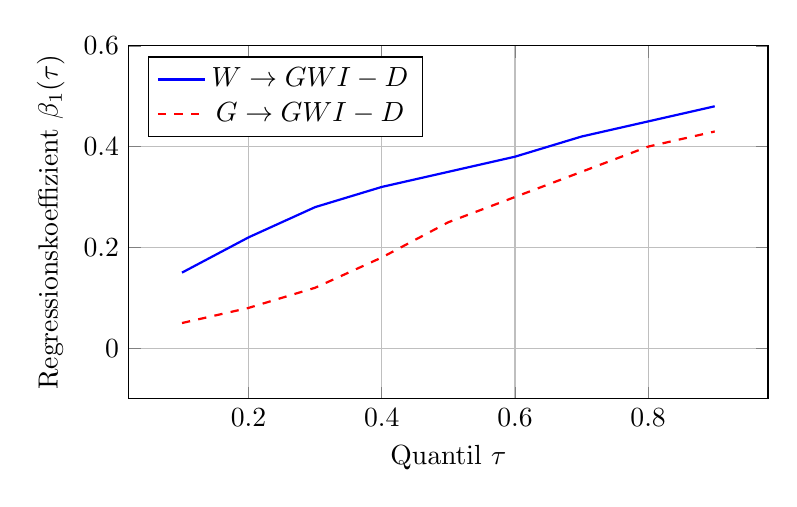
\begin{tikzpicture}
    \begin{axis}[
      width=0.8\textwidth,
      height=0.5\textwidth,
      xlabel={Quantil \(\tau\)},
      ylabel={Regressionskoeffizient \(\beta_1(\tau)\)},
      ymin=-0.1, ymax=0.6,
      grid=both,
      legend pos=north west,
      ]
      \addplot[color=blue, thick] coordinates {
        (0.1,0.15) (0.2,0.22) (0.3,0.28) (0.4,0.32) (0.5,0.35) (0.6,0.38) (0.7,0.42) (0.8,0.45) (0.9,0.48)
      };
      \addplot[color=red, dashed, thick] coordinates {
        (0.1,0.05) (0.2,0.08) (0.3,0.12) (0.4,0.18) (0.5,0.25) (0.6,0.30) (0.7,0.35) (0.8,0.40) (0.9,0.43)
      };
      \legend{\(W \rightarrow GWI-D\), \(G \rightarrow GWI-D\)}
    \end{axis}
  \end{tikzpicture}
  \caption{Quantilregressionskoeffizienten für den Einfluss von \(W\) und \(G\) auf den GWI-D}
  \label{fig:quantilregression}
\end{figure}

Abbildung \ref{fig:quantilregression} zeigt die geschätzten Koeffizienten einer Quantilregression, bei der der Einfluss der Wirtschafts- (\(W\)) und Gerechtigkeitskomponente (\(G\)) auf den aggregierten GWI-D über verschiedene Quantile \(\tau\) modelliert wird. Beide Kurven weisen einen positiven Anstieg auf, d.h. der Einfluss beider Komponenten auf den Gesamtindex ist in den oberen Quantilen stärker ausgeprägt als in den unteren. Dies deutet darauf hin, dass bereits hohe Ausgangswerte in \(W\) oder \(G\) den GWI-D überproportional stärker positiv beeinflussen – ein Hinweis auf mögliche „wohlfahrtsverstärkende“ Effekte.

\section{Paarweise Korrelationen}

\begin{table}[ht]
  \centering
  \caption{Paarweise Korrelationskoeffizienten zwischen GWI-D Komponenten}
  \label{tab:korrelationen}
  \begin{tabular}{lcccc}
    \toprule
    & \textbf{W (\(W\))} & \textbf{G (\(G\))} & \textbf{Z (\(Z\))} & \textbf{S (\(S\))} \\
    \midrule
    \textbf{W (\(W\))} & 1.00 & 0.45 & 0.78 & 0.62 \\
    \textbf{G (\(G\))} & 0.45 & 1.00 & 0.52 & 0.31 \\
    \textbf{Z (\(Z\))} & 0.78 & 0.52 & 1.00 & 0.58 \\
    \textbf{S (\(S\))} & 0.62 & 0.31 & 0.58 & 1.00 \\
    \bottomrule
  \end{tabular}
  \vspace{0.2cm}
  \footnotesize{\textit{Anmerkung: Alle Korrelationen signifikant bei p < 0,01.}}
\end{table}

Die paarweisen Beziehungen zwischen den Komponenten werden in Tabelle \ref{tab:korrelationen} quantifiziert. Besonders stark ist der lineare Zusammenhang zwischen \(W\) und \(Z\) (Korrelationskoeffizient \(r = 0{,}78\)), was auf eine enge Verknüpfung von wirtschaftlicher Leistungsfähigkeit und Zukunftsorientierung hindeutet. Interessant ist die vergleichsweise schwache Korrelation zwischen \(G\) und \(S\) (\(r = 0{,}31\)), was darauf hindeutet, dass soziale Gerechtigkeit und gesellschaftlicher Zusammenhalt nicht automatisch Hand in Hand gehen.

\section{Zusammenfassung und Interpretation}

Die Verteilungsanalyse der GWI-D Komponenten erlaubt folgende Schlussfolgerungen:

\begin{enumerate}
  \item \textbf{Wirtschaft (\(W\))} zeigt die höchste Volatilität und ist besonders anfällig für konjunkturelle und krisenbedingte Schwankungen.
  \item \textbf{Gerechtigkeit (\(G\))} weist den niedrigsten Mittelwert auf und zeigt eine signifikant nicht-normalverteilte, linksschiefe Verteilung.
  \item \textbf{Zukunft (\(Z\))} korreliert stark mit der Wirtschaftskomponente, was die Bedeutung ökonomischer Grundlagen für langfristige Perspektiven unterstreicht.
  \item \textbf{Zusammenhalt (\(S\))} ist die stabilste Komponente mit geringer zeitlicher Variabilität, zeigt jedoch in der jüngsten Multikrise erste Erosionszeichen.
  \item Die \textbf{Quantilregression} offenbart, dass bereits hohe Werte in einzelnen Dimensionen den Gesamtindex überproportional positiv beeinflussen – ein Hinweis auf positive Synergieeffekte zwischen den Säulen.
  \item Die \textbf{schwache Korrelation zwischen Gerechtigkeit und Zusammenhalt} (\(r = 0{,}31\)) deutet auf einen potenziellen Zielkonflikt hin: Mehr soziale Gerechtigkeit führt nicht automatisch zu stärkerem gesellschaftlichem Zusammenhalt.
\end{enumerate}

Diese Befunde legen nahe, dass eine nachhaltige Gemeinwohlorientierung nicht nur auf eine einzelne Dimension abzielen darf, sondern integrative Politiken erfordert, die alle vier Säulen gleichermaßen stärken. Besondere Aufmerksamkeit verdient dabei die Gerechtigkeitskomponente, die trotz langfristiger Verbesserungen weiterhin das schwächste Glied in der Kette darstellt. Die identifizierte Diskrepanz zwischen Gerechtigkeit und Zusammenhalt erfordert zudem gezielte Maßnahmen, um beide Ziele synchron zu verfolgen.

\endinput